% case name
\chapter{solit}
%
% - Purpose & Description:
%     These first two parts give reader short details about the test case,
%     the physical phenomena involved, the geometry and specify how the numerical solution will be validated
%

\section{Purpose}
%
This test demonstrates the ability of \telemac{3d} to model the
propagation of a solitary wave with only 2, 3 or 4 vertical levels.
In an ideal case, the wave should travel without changing its shape and amplitude.
This study demonstrates the necessity of using the non-hydrostatic
version of the software to simulate non-linear waves propagation.
%
\section{Notations}

This test-case is the same as described in \cite{Jankowski1999}. The notations
are illustrated in the Figure \ref{fig:solit_notations}.

\begin{figure}[H]
\begin{center}
  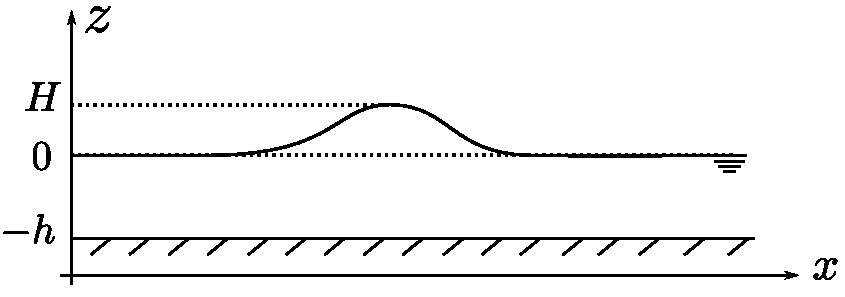
\includegraphics[scale=0.7]{img/figure1.pdf}
\end{center}
\caption{Solitary wave propagation over a flat bottom: description of the notations.}
\label{fig:solit_notations}
\end{figure}


\section{Theory}

\begin{WarningBlock}{Authorship}
The following description is extracted from the PhD thesis of Jacek A. Jankowski \cite{Jankowski1999}.
Only slight changes were done to the text.
\end{WarningBlock}

A solitary wave is a single elevation of the water surface above an undisturbed surrounding,
which is neither preceded nor followed by any free surface disturbances. Neglecting
dissipation, as well as bottom and lateral boundary shear, a solitary wave travels over a
horizontal bottom without changing its shape and velocity.
The accuracy of the model can be evaluated by comparing the
amplitude and celerity of the wave with its theoretical values, as well as the deformation
of the wave as it travels.\\

There are several theories that aim at giving an approximation of the free-surface and velocity
field for this form of non-linear finite-amplitude wave. The most known ones are the Stokes and cnoïdal
waves theories. The latter is used here, based on Laitone \cite{Laitone1960}. According to \cite{Jankowski1999}, it
is the most frequently used for comparative studies.
It provides approximate formulae for the
velocity components $u$, $w$, free surface elevation $\eta$ defined as $\eta = z + h$,
pressure $p$ and wave celerity $c$ of a
solitary wave with a height of $H$, on a vertical section of an infinitely long channel of an undisturbed
depth $h$ ($z = 0$ at the free-surface, see the Figure \ref{fig:solit_notations}). They read:
\begin{equation}
\label{eq:solit}
\left\{\begin{array}{l}
u = \sqrt{gh}\dfrac{H}{h}\text{sech}^2\left[\sqrt{\dfrac{3}{4}\dfrac{H}{h^3}(x-ct)}\right] \medskip \\
w = \left(\sqrt{3gh}\sqrt{\dfrac{H}{h^3}}\dfrac{z+h}{h}\right)\text{sech}^2\left[\sqrt{\dfrac{3}{4}\dfrac{H}{h^3}(x-ct)}\right]
\text{tanh}\left[\sqrt{\dfrac{3}{4}\dfrac{H}{h^3}(x-ct)}\right] \medskip \\
\eta = h+H\text{sech}^2\left[\sqrt{\dfrac{3}{4}\dfrac{H}{h^3}(x-ct)}\right] \medskip \\
p= \rho g (\eta + z) \medskip \\
c = \sqrt{g(H+h)}
\end{array}\right.
\end{equation}
It is interesting that in this analytical approximation the vertical velocity component is
not treated as small, as commonly taken, but the pressure can be assumed hydrostatic
(fourth line of \eqref{eq:solit}) at the same level of exactness as the horizontal velocity
(with $\mathcal{O}((H/h)^2)$)\cite{Laitone1960}.
Therefore, this initial condition is suitable for fair comparisons between models
with and without hydrostatic approximation and the initial value of zero hydrodynamic
pressure is assumed. Although the initial velocity field (first two lines of \eqref{eq:solit})
is perfectly divergence-free, larger values of the hydrodynamic pressure appear immediately after the first time
step (60\% of the value of the hydrostatic pressure at the bottom).\\

Following the test cases provided by Ramaswamy \cite{Ramaswamy1990}, a solitary wave described by
\eqref{eq:solit} is applied in a long channel as an initial condition, and the
behaviour of the solution is observed thereafter. Due to the fact that the simulation is
performed in a finite domain, and Laitone’s formulae are valid for an indefinitely long
channel, care must be taken choosing the initial position of the wave crest. In order to
deal with it, the use of the effective wave length $\lambda$ concept is made. $\lambda$ is equal to the
doubled length between the wave crest and a point, where the free surface elevation is
$\eta(x) = 0.01H$. According to Laitone:
\begin{equation}
\lambda = 6.9\sqrt{\dfrac{h^3}{H}}
\end{equation}
For example, when $H/h = 0.1$, $\lambda/2 \approx 11h$, and for a channel of $10 m$ depth, the initial
distance between the solitary wave crest and a boundary should be at least $110 m$.
%The steepness of the solitary wave grows with $H/h$.
%As the solitary wave travels along a
%shoaling bottom, its height $H$ increases, until wave breaking appears. As the criterion
%for wave breaking the critical condition is assumed when the particle velocity at the crest
%equals the wave celerity. Various approximations yield values for maximum solitary wave
%height between $H = 0.727h$ and $H = 0.827h$ \cite{[113, 95]}.

\section{Description}
%
%
% - Geometry and Mesh:
%     This part describes the mesh used in the computation
%
\subsection{Geometry and Mesh}

\subsubsection{Geometry}
A long channel of $600 m$ long and $6 m$ wide is considered, with a constant depth $h = 10 m$.
The bottom is flat, at the elevation $z = -10m$.

\subsubsection{Mesh}
The mesh is composed of 6 elements on the width and 600 on the length,
with a resolution in the direction parallel to the channel axis of $1 m$ (see the Figure \ref{fig:solit_mesh}).
This corresponds to 7,206 triangular elements and 4,210 nodes.
Various numbers of planes on the vertical are considered: 2, 3 and 4.
\begin{figure}[H]
\begin{center}
  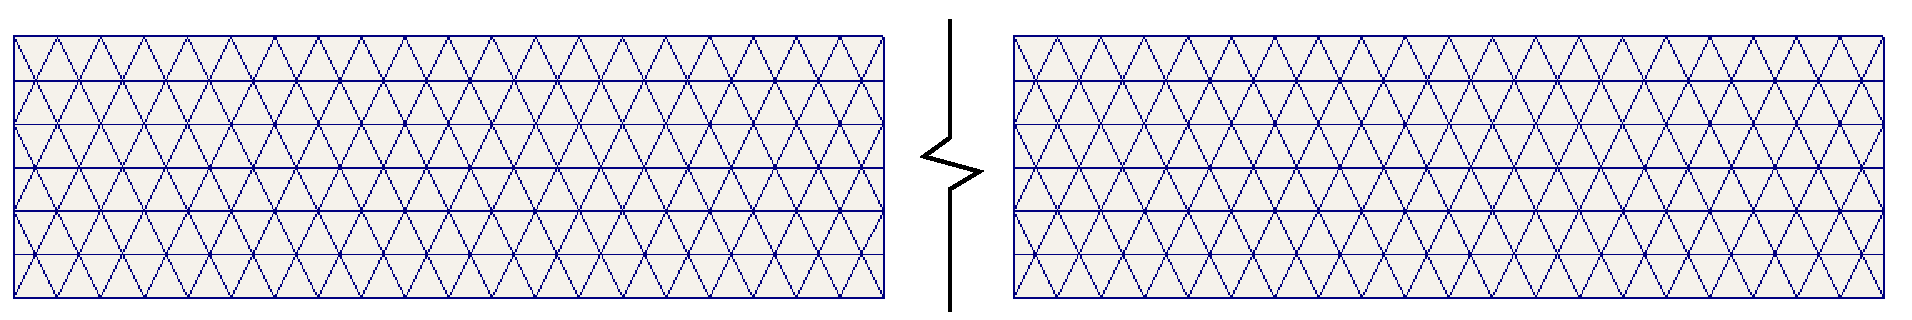
\includegraphics[scale=0.45]{img/figure2.pdf}
\end{center}
\caption{Solitary wave propagation over a flat bottom: mesh of the case in the $(x,y)$ plane.}
\label{fig:solit_mesh}
\end{figure}

\subsection{Physical parameters}
%
The flow is assumed to be inviscid, without shear on the lateral boundaries and on the bottom.
%
\subsection{Initial and Boundary Conditions}
%
\subsubsection{Initial conditions}
%
As the initial condition the hydrostatic approximation
given by \eqref{eq:solit} is applied, with a wave height of $H = 1 m$,
and the initial crest position at $x = 150 m$. The velocity field and the free-surface
elevation are given by \eqref{eq:solit}.
%
\subsubsection{Boundary conditions}
%
The lateral boundaries and the bottom are impervious, there is no friction.
%
\subsection{General parameters}
%
The time step size is constant, equal to $\Delta t = 0.1 s$ (the Courant number in the direction
of wave propagation varies from $0.2$ to about $1.0$ at the wave crest).
The simulation time is $30 s$.

\subsection{Numerical parameters}
%
The non-hydrostatic version is used. Advection of velocities is done with the method of characteristics.
The solver for the pressure is a conjugate gradient with diagonal preconditionning,
an accuracy of $1e-6$ is asked for with a maximum number of iterations of 500.
A coefficient of implicitation for the depth and velocities of 0.51 is used.
A mass-lumping is used on the depth, with a cofficient of 1.
There are no tidal flats in this case.
%
\section{Results}
%
\begin{figure}[H]
\begin{center}
  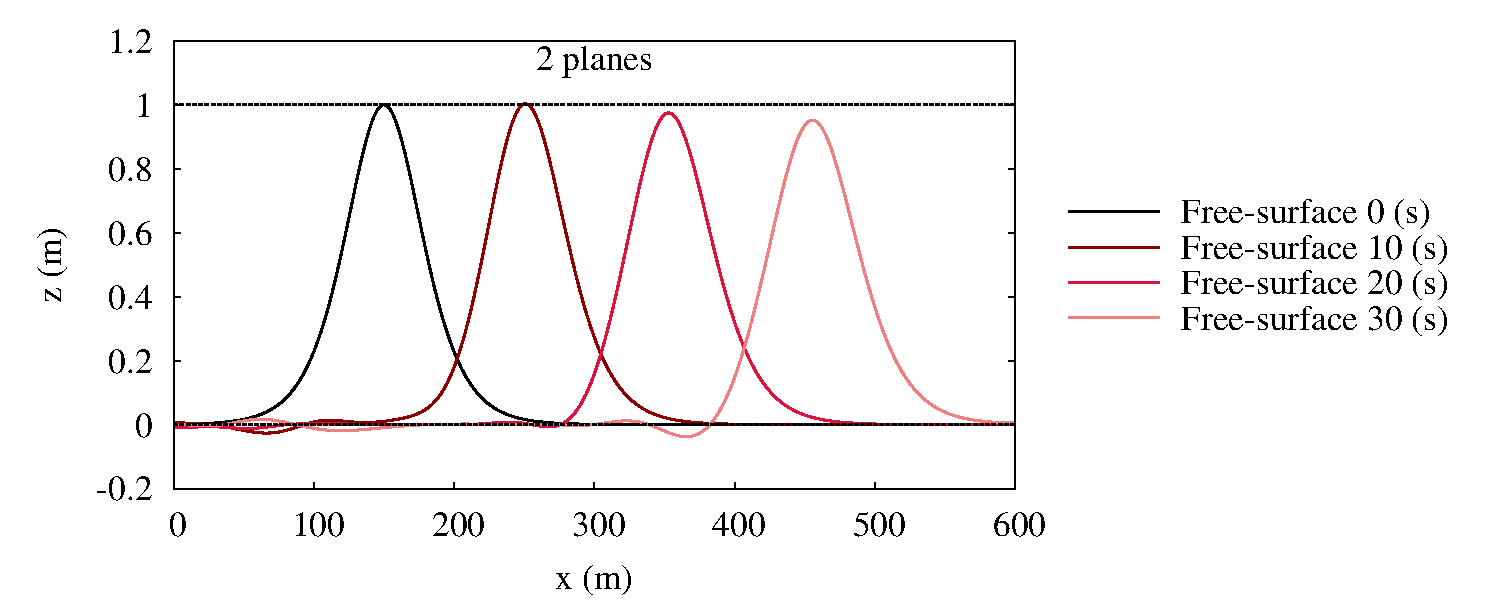
\includegraphics[scale=0.6]{img/figure3a.pdf}
  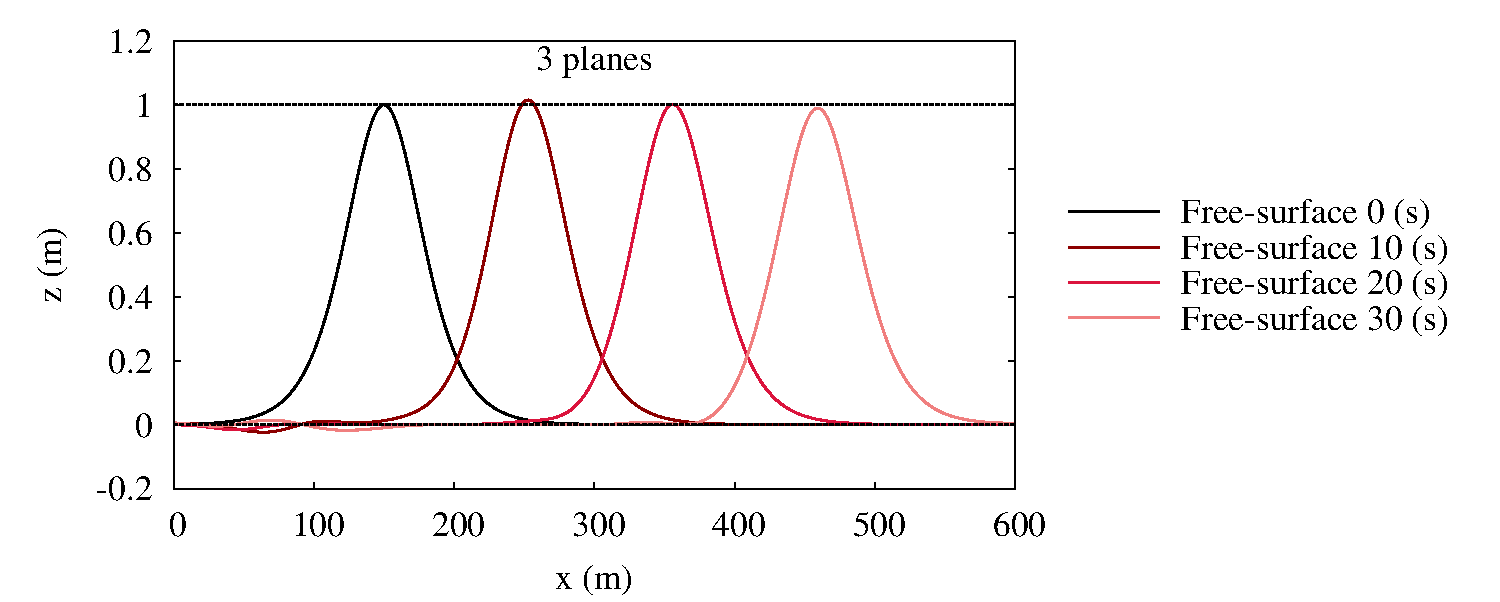
\includegraphics[scale=0.6]{img/figure3b.pdf}
  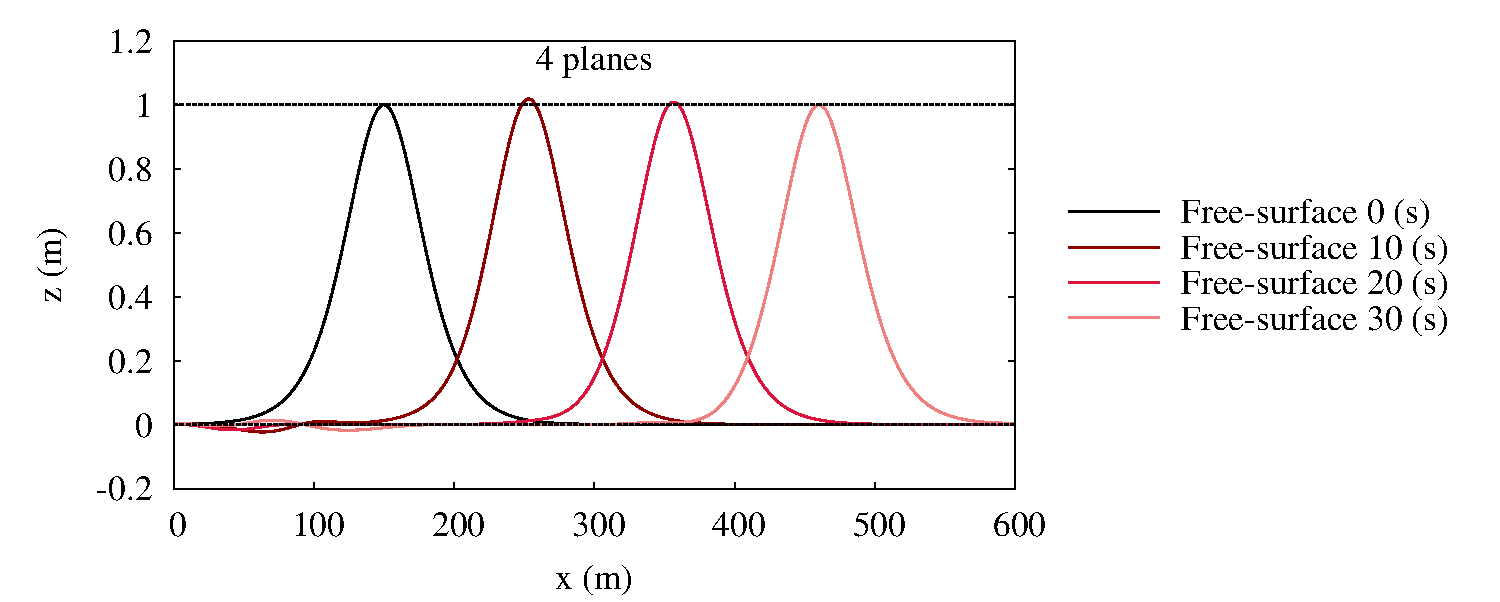
\includegraphics[scale=0.6]{img/figure3c.pdf}
\caption{Solitary wave propagation over a flat bottom: simulation results using 2, 3 and 4 planes.}
\label{fig:solit_results}
\end{center}
\end{figure}
%
Figure \ref{fig:solit_results} presents a longitudinal cross profile of the free surface
at different times of the simulation and for the various configurations
on vertical discretisation.
The amplitude of the wave remains nearly constant in all cases.
The relative error on the wave amplitude after $30s$ is of 4.8\% with 2 planes and about 0.01\%
with 3 and 4 planes (see the Table~\ref{tab:solit_celerity}).
On the other hand, the theoretical celerity of the propagation is equal to $\sqrt{g(h+H)}$.
With a water level $h = 10m$ and a wave height $H=1m$,
the theoretical celerity is equal to $10.38ms^{-1}$.
Table~\ref{tab:solit_celerity} shows the values of the wave displacement and celerity
on the numerical models (using 2, 3 and 4 planes). The error on the celerity is also
displayed, showing a maximum error of 1.9\% (using two planes) and less than 1\% when refining on the vertical.
\begin{table}[H]
\caption{Solitary wave propagation over a flat bottom:
values of the wave height and displacement after $30s$ in the simulation,
together with the values of wave celerity and relative error on the celerity
using 2, 3 and 4 planes in the mesh.}
\label{tab:solit_celerity}
\begin{center}\begin{tabular}{|c|c|c|c|}
\hline
~ & \textbf{2 planes} & \textbf{3 planes} & \textbf{4 planes}\\
\hline
\textbf{Final wave height ($m$)} & 0.952 & 0.999875 & 1.0002 \\
\hline
\textbf{Final displacement ($m$)} & 305.5 & 309 & 310 \\
\hline
\textbf{Wave celerity ($ms^{-1}$)} & 10.18 & 10.3 & 10.33 \\
\hline
\textbf{Relative error on the celerity (\%)} & 1.9 & 0.8 & 0.5 \\
\hline
\end{tabular}\end{center}
\end{table}
\begin{WarningBlock}{Results using the hydrostatic version of TELEMAC-3D}
The users should be aware that when using the hydrostatic version on this test-case, the
results are not in good agreement with the approximate theoretical solution: the shape of the velocity field
is deteriorated, the error on the wave celerity is of about 10\% and the error on the wave height after $30s$
of propagation is of 15\%.
\end{WarningBlock}
%\begin{table}[H]
%\caption{Solitary wave propagation over a flat bottom:
%values of the wave height and displacement after $30s$ in the simulation,
%together with the values of wave celerity and relative error on the celerity
%using the non-hydrostatic and hydrostatic versions with 4 planes.}
%\label{tab:solit_celerity}
%\begin{center}\begin{tabular}{|c|c|c|c|}
%\hline
%~ & \textbf{Hydrostatic} & \textbf{Non-hydrostatic} & \textbf{Non-hydrostatic -- dynamic pressure in wave equation}\\
%\hline
%\textbf{Final wave height ($m$)} & 1.14966 & 1.0002 & 1.00562 \\
%\hline
%\textbf{Final displacement ($m$)} & 342 & 310 & 307.5 \\
%\hline
%\textbf{Wave celerity ($ms^{-1}$)} & 11.4 & 10.33 & 10.25 \\
%\hline
%\textbf{Relative error on the celerity (\%)} & 9.8 & 0.5 & 1.3 \\
%\hline
%\end{tabular}\end{center}
%\end{table}
%
\section{Conclusion}
%
\telemac{3d} correctly simulates the propagation of a solitary wave when using the non-hydrostatic formulation.
